%%-*-Latex-*-
\mychapter{Program Overview --- The Fundamentals}
\label{chap:overview}

This chapter presents the reader with a first glimpse into the world of \PSD
It is clearly important when one is trying to get to grips with a code of the
proportions of \PS to be able to visualise the main aspects of the device
being simulated at an early stage, without too much detail obscuring the
overall picture. Similarly it is important to provide the potential users with
an overview of the code structure and its operation before they embark on a
closer study. The aim of this chapter is to aid this visualisation by
presenting a brief description of the machine, its subsystems and the code
layout in simple, general terms. Chapter~\ref{chap:models} will provide users
with more detail about how to customise the models and parameters mentioned
here.

\section{The Machine}

A natural starting point for a systems code manual is the description of the
system itself. In this case, the (default) system is a tokamak fusion power
plant, modelled using a large number of equations based on knowledge of the
underlying physics and engineering models of each subsystem of the machine. As
will be emphasised later the bulk of the program is ordered into modules
roughly corresponding to each of the subsystems, so an early attempt at
familiarising the reader with them will hopefully be of some benefit.

\subsection{Radial and Vertical Build}
Figure~\ref{fig:build1} shows schematically the layout of a typical tokamak as
modelled by \PSD This is the so-called `build' of the machine --- the relative
locations of the major components. Their positions are referenced to the
$(R,Z)$ coordinate system, where $R$ is the radial distance from the vertical
centreline (axis) of the torus, and $Z$ is the vertical distance from the
equatorial midplane, about which the machine is assumed to be up-down
symmetrical. Components are often referred to as being `inboard' or
`outboard', which simply means that they lie at a radius $R$ less than or
greater than $R_0$, respectively, where $R_0$ is the plasma major radius ({\tt
rmajor}).

\begin{figure}
\centerline{\epsfig{file=BUILD1.ps,width=160mm,height=160mm,
bbllx=0mm,bburx=200mm,bblly=0mm,bbury=200mm,clip=}}
\vspace{-12mm}
\caption[build1] {\it Schematic diagram of the fusion power core of a typical
tokamak power plant modelled by \PSC showing the relative positions of the
components. The numbers shown in the PF coil blocks are the values of the {\tt
ipfloc} switch for that block.}
\label{fig:build1}
\end{figure}

Figure~\ref{fig:build2} shows the \FORT variables that describe the
thicknesses and positions involved. It must be emphasised that these two
figures are very much schematic, otherwise they could become slightly
misleading. For the sake of clarity the thicknesses are not drawn to scale,
and the space labelled as the divertor does not indicate in any way the actual
shape of that component. The cryostat acts as a dewar or vacuum vessel, and is
therefore continuous in reality, enclosing all of the components within
it. Only in the code's build calculation is there an apparent gap in the
cryostat beneath the top of the TF coil.

\begin{figure}
\centerline{\epsfig{file=BUILD2.ps,width=160mm,height=160mm,
bbllx=0mm,bburx=200mm,bblly=0mm,bbury=200mm,clip=}}
\vspace{-12mm}
\caption[build2] {\it Schematic diagram of the fusion power core of a typical
tokamak power plant modelled by \PSC showing the variables used to define the
thicknesses of the components. The arrowed labels adjacent to the axes are the
total `builds' to that point. The precise locations and sizes of the PF coils
are calculated within the code.}
\label{fig:build2}
\end{figure}

Most of the thicknesses shown in Figure~\ref{fig:build2} are input parameters,
so are not changed during the course of the simulation.  The rest are
calculated by the code during execution. In addition, some of the component
sizes can be used as {\it iteration variables}\/ (see
Section~\ref{sec:itvars}) to help in the optimisation process.

\subsection{Principal Components}

\subsubsection{Plasma}
Arguably, the most important component of the machine is the plasma
itself. This is assumed to have an up-down symmetric, double null
configuration, with elongation and triangularity specified by the user. A
great number of physics models are coded within \PS describing the behaviour
of the plasma parameters such as its current, temperature, density, pressure,
confinement etc., and also the various limits that define the stable operating
domain.

\subsubsection{Scrape-off Layer}
The region directly outside the last closed flux surface of the plasma is
known as the scrape-off layer, and contains no structural material.  Plasma
entering this region is not confined and is removed by the divertor. \PS
treats the scrape-off layer merely as a gap.

\subsubsection{First Wall}
The first wall acts as a physical barrier protecting the rest of the machine
from the hot plasma. Due to its hostile environment the first wall has only a
short lifetime and therefore needs to be replaced regularly. Its stainless
steel structure is cooled either by gaseous helium or by pressurised water.

\subsubsection{Divertor}
The divertor provides a means of removing plasma reaching the scrape-off layer
and heavy ions that are ejected from the first wall.  Two divertors are
assumed in the \PS tokamak, placed symmetrically above and below the plasma
(N.B.\ see Section~\ref{sec:divmod}). The principal outputs from the code
are the divertor heat load, used to determine its lifetime, and its peak
temperature. The divertor is cooled either by gaseous helium or by pressurised
water.

\subsubsection{Blanket}
The blanket performs a number of tasks. An incoming neutron from a
deuterium-tritium (D-T) fusion reaction in the plasma loses energy in the
blanket. This energy is removed by the blanket coolant and used to produce
electricity. The neutron may also react with a lithium nucleus present in the
blanket to produce a tritium nucleus which can be re-used as fuel. The
competing requirements of heating and tritium synthesis mean that a neutron
multiplier must be present, to ensure balance between tritium destruction and
creation. The blanket therefore contains beryllium to fulfil this
purpose. Again, the blanket has a relatively short lifetime because of the
high neutron fluence. Steel and vanadium may be used as structural materials
within the blanket, which is cooled either by gaseous helium or by pressurised
water.

\subsubsection{Shield}
The stainless steel shield reduces the neutron flux reaching the TF coils and
beyond. This minimises the radiological impact of the neutrons, and their
heating of the TF coils which, if superconducting, need to remain at liquid
helium temperatures. The shield is cooled either by gaseous helium or by
pressurised water, and as with the blanket the energy deposited in the coolant
is used to produce electricity.

\subsubsection{TF Coils}
The toroidal field (TF) coils can be either resistive or superconducting. In
the superconductor model, the CICC (Conductor In Cable Conduit) structure
shown in Figure~\ref{fig:CICC} is used, and the coils are cooled using a
liquid helium cryogenic system. Among the TF coil parameters calculated by the
code are the maximum allowable current density, the stresses on the structure,
the energy stored and the magnetic field produced by the coils.

The current in the TF coils must be sufficient to produce the right toroidal
field at the centre of the plasma. The field falls off at a rate $1/R$, with
the peak value occurring at the outer edge of the inboard portion of the TF
coil ($R_{\mbox{\scriptsize max TF}} = \mbox{\tt rbmax}$). The maximum TF coil
current depends on the field it produces and the allowable current density.

Each TF coil is defined in the $(R,Z)$ plane by four circular arcs of
different radius, which create a D-shaped profile. Because of the finite
number of TF coils used in a tokamak (typically around 20), the toroidal field
has a ripple introduced into it, the amplitude of which can be limited to a
few per cent by the code by adjusting the outboard gap thickness (labelled
{\tt gapsto} in Figure~\ref{fig:build2}).  Ports are often necessary for
auxiliary power systems etc., and the gaps between adjacent TF coils can be
made large enough to accommodate such equipment.

\begin{figure}
\centerline{\epsfig{file=CICC.ps,width=160mm,height=160mm,
bbllx=0mm,bburx=210mm,bblly=0mm,bbury=210mm,clip=}}
\vspace{-12mm}
\caption[CICC]
{\it Schematic diagram of the cross-section of a superconducting TF coil,
showing the CICC (Conductor In Cable Conduit) construction. The cable space
contains superconducting filaments and circulating liquid helium coolant.}
\label{fig:CICC}
\end{figure}

\subsubsection{Bucking Cylinder}
The bucking cylinder provides some strength to the inboard TF coil
structure. If the TF coils are superconducting, the bucking cylinder is cooled
by the cryogenic system.

\subsubsection{Cryostat}
The cryostat acts as a dewar and vacuum vessel, and is used to cool those
components that need to operate at liquid helium temperatures. These include
any superconducting (TF or PF) coils, the inter-coil structure and the bucking
cylinder. \PS calculates the cryogenic power load and the resulting heat
exchanger requirements. As stated earlier, the build picture in
Figure~\ref{fig:build1} is slightly misleading in that the cryostat completely
encloses the components within it --- there is no large gap beneath the TF
coil as is the case in Figure~\ref{fig:build1}.

In addition to this (inner) cryostat, an external cylindrical dewar encloses
the whole of the tokamak.

\subsubsection{PF Coils}
The poloidal field (PF) coils can be either resistive or superconducting, and
are used initially to cancel the vertical field produced at the centre of the
plasma by the OH coil during start-up, and then to maintain the plasma
position and shape during the flat-top period. The positions and sizes of the
PF coils are partly input, and partly calculated after consideration of the
required currents and allowable current density. The PF coils are generally
grouped into up-down symmetric pairs, and each group can be placed in one of
three regions, either vertically above (and below) the OH coil ({\tt
ipfloc(i)=1}), vertically above (and below) the TF coil ({\tt ipfloc(i)=2}),
or radially outside the TF coil ({\tt ipfloc(i)=3}).

The PF coil currents vary as a function of time during the tokamak operation
as indicated in Figure~\ref{fig:current_vs_time}.

\begin{figure}
\centerline{\epsfig{file=IVST.ps,width=160mm,height=160mm,
bbllx=0mm,bburx=200mm,bblly=0mm,bbury=200mm,clip=}}
\vspace{-12mm}
\caption[IvsT]
{\it Plot showing schematically the current waveforms for the plasma, a
typical PF coil, and the OH coil.}
\label{fig:current_vs_time}
\end{figure}

\subsubsection{OH Coil}
The ohmic heating (OH) coil is a PF coil used primarily during start-up (but
also during the burn phase) to create and maintain the plasma current by
inductive means. Swinging (changing) the current through the OH coil causes a
change in the flux linked to the plasma region, inducing a current in it. \PS
calculates the amount of flux required to produce the plasma current, and also
the amount actually available. The code measures the magnetic flux in units of
Volt-seconds ($=$ Webers). The OH coil is sometimes referred to as the central
solenoid, and can be either resistive or superconducting.

\subsubsection{Auxiliary Power Systems}
The use of purely inductive current drive leads to pulsed plant operation
because of the limited flux swing that can be achieved using the OH coil. This
poses problems due to the fact that fatigue failures may result, and there
would also be a need for thermal storage to maintain a level supply between
pulses. However, the plasma current can also be produced and maintained
(partially or wholly) using non-inductive means which, in principle, removes
this restriction. \PS contains a number of auxiliary current drive schemes,
including various RF methods (Lower Hybrid, Electron Cyclotron, and Ion
Cyclotron (Fast Wave) current drives) and also Neutral Beam current drive
systems. The code calculates the efficiency and the resulting power
requirements of the chosen system.

\subsubsection{Structural Components}
Structural components are required to provide support for the fusion power
core systems against gravity and the magnetic forces that will be encountered
during operation. The required structural masses and their costs are
calculated.

\subsubsection{Power Conversion and Heat Dissipation Systems}
The \PS power plant takes into account all the systems required to perform the
necessary conversion of fusion power to electricity, from the coolant systems
in the plant components to the heat exchangers and turbines.
Figure~\ref{fig:pwrconv} shows schematically the overall power transfer
mechanisms used by the code.

\begin{figure}
\centerline{\epsfig{file=PWR.ps,width=160mm,height=160mm,
bbllx=0mm,bburx=200mm,bblly=0mm,bbury=200mm,clip=}}
\vspace{-12mm}
\caption[PWRCONV]
{\it Schematic diagram showing the power conversion mechanisms used in \PS
\cite[Note 0166]{PWF}.}
\label{fig:pwrconv}
\end{figure}

\subsubsection{Vacuum Systems}
The vacuum system is used for four different processes. Firstly, before plasma
operations the chamber must be evacuated to remove outgassed impurities from
the structure. Secondly, the chamber must be re-evacuated between burn
operations. Thirdly, helium ash must be removed to prevent it from diluting
the fuel. Finally, deuterium and tritium is removed on a steady state
basis. \PS calculates the parameters of a vacuum system that satisfy all four
requirements, with the option of either turbo pumps or cryo pumps being used.

\subsubsection{Buildings}
The volume and ground area of all the various buildings on a power plant site
are included in the \PS calculations for the benefit of the costing
algorithms.

\subsection{Tight Aspect Ratio Tokamaks}

\PS has the ability to perform studies on tokamaks in the low aspect ratio
regime (major radius $\leq 2 \times$ minor radius). The physics and
engineering issues~\cite{tart} associated with these machines are somewhat
different from those of conventional aspect ratio, and this is reflected by
the following special models~\cite{storac} in \PSD
\begin{enumerate}
\item The inboard build of a TART is very different from that in a
conventional tokamak. There is no inboard blanket (and possibly no inboard
shield), and the inboard TF coil legs are replaced by a single centrepost.
\item The centrepost is constructed from copper (as are the outboard TF coil
sections), and is tapered so that it is narrowest at the midplane of the
device. The parameters of the centrepost coolant system are calculated by \PSC
including the pump pressure, maximum temperature and pipe radius.
\item A gaseous divertor model is used, and a simple divertor heat load
calculation is employed.
\item A simple PF coil current scaling algorithm is available for use with the
TART option.
\item The plasma shaping terms (elongation and triangularity) can be
calculated directly given the aspect ratio.
\item Among the physics models that differ from those relevant to conventional
aspect ratio machines are (i) the bootstrap current fraction, (ii) the Troyon
beta limit, and (iii) the neutron heating of the centrepost.
\end{enumerate}
Since \PS is set up by default to deal with conventional aspect ratio
machines, TART power plants will only be referred to briefly in the rest of
this manual.

\subsection{D-$^3$He Tokamaks}

In addition to the standard deuterium-tritium fusion reaction
(Equation~\ref{eq:d-t}), \PS can also investigate power plants that utilise
the deuterium-$^3$helium reaction (Equation~\ref{eq:dhe3}). The fusion
reaction rate is significantly different from that for D-T fusion, and the
power flow from the plasma is modified since charged particles are produced
rather than neutrons.

D-$^3$He tokamak power plants do not include blankets, because of the near
absence of neutrons leaving the plasma, and the fact that no tritium needs to
be produced for fuel.

\subsection{Pulsed Plant Scenario}

If the plasma current is not to be driven by purely non-inductive means, it is
necessary to operate the plant in a pulsed manner as the current swing in the
OH/PF coils cannot be continued indefinitely. \PS can perform a number of
calculations relevant to a pulsed power plant, as summarised below.

\subsubsection{Thermal Cycling Package}
This performs calculations on the first wall of the machine. Evaluation of the
mechanical and thermal stresses on this component lead to a measure of the
maximum number of cycles to which the first wall can be subjected, and hence
to the minimum allowable length of each reactor cycle for a specified first
wall lifetime. The thickness of the first wall is constrained to lie within
lower and upper bounds, which ensures that it can withstand the internal
coolant pressure and the peak temperature and neutron fluence.

\subsubsection{OH Coil Swing Time}
This calculation ensures that the plasma current ramp rate during start-up is
prevented from being too high, as governed by the requirement to maintain
plasma stability in $l_i$ - $q_\psi$ space.

\subsubsection{Burn Time}
The length of the burn time is calculated from the surplus volt-seconds
available from the OH/PF coil system during the plasma burn phase, after the
flux required during the plasma start-up is taken into account.

\subsubsection{Start-up Power Requirements}
The minimum auxiliary power required during the start-up (ignition) phase is
calculated on the basis of a POPCON analysis. Ignition is accessed via the
so-called Cordey Pass (the path in plasma density--temperature space which
minimises the power requirement) and the code ensures that there is sufficient
auxiliary power to accommodate this. In fact, this calculation is very
CPU-intensive, so the relevant routine is not called at present. In practice,
the auxiliary power tends to exceed the minimum allowable value anyway,
without any need to constrain it to do so.

\subsubsection{Thermal storage}
Three options for providing the thermal storage required to maintain the
machine's output during the off-periods are available. The first relies on the
thermal storage inherent in the machine's steam cycle, the second incorporates
an extra boiler to boost the thermal storage, and the third relies on a large
stainless steel block acting as the thermal storage medium. The costs of these
three options are added to the relevant cost accounts.

\subsection{Safety and Environment Models}
At present, the neutronics, activation and inventory calculations comprise the
safety and environment models in the code. These will be extended as a result
of forthcoming work.

\subsubsection{Neutronics}
The neutronics module predicts the neutron flux spectra in the inboard and
outboard first wall and blanket components. The spectra are based on a
simplified tokamak device that has a fixed ratio ($=1.5825$) between the
outboard blanket thickness and the inboard blanket thickness, and are scaled
according to the actual thickness of the outboard blanket. This relatively
limited, single-parameter approach is expected to be replaced by a more
general method, which should allow a more accurate portrayal of the device
being modelled by \PSD

\subsubsection{Activation and Inventory Information}
The code evaluates the consequences of exposing the power plant's materials to
the calculated neutron fluxes, subject to the limitations imposed by the
neutronics module. A library of neutron cross-sections and decay data is used
to calculate the total activity, gamma-ray dose rate and decay heat output due
to the materials' exposure to neutrons, both at the end of the plant's life
and at a time 100 years later. These values are relevant to decommissioning
and disposal studies, and additional parameters that can be obtained from the
nuclide inventory will also be included as the need arises.

\subsection{Stellarator Model}
The code has the ability to perform calculations based on the physics and
engineering of a stellarator, which, although being a toroidal device, is
radically different in a number of ways from a tokamak.

The model is derived from two main sources; the physics is based on that
assumed by the U.S.\ stellarator reactor study group~\cite{USSRSG}, and the
coil set is scaled from the proposed Wendelstein VII-X design, a modular
advanced stellarator with a 5-period Helias configuration~\cite{W7X}.

\subsubsection{Physics Models}
Much of the physics is identical to that for tokamaks, including the plasma
composition, fusion power considerations and energy conversion and transport
within the plasma. However, some physics topics do differ between stellarators
and tokamaks:
\begin{enumerate}
\item Plasma current scaling: Stellarators have zero plasma current, so no
current scalings are required.
\item Heating/current drive: Stellarators require no current drive, although
provision for auxiliary heating does need to be present.
\item Density and beta limits: Stellarator-relevant plasma limits are
available within the code.
\item $\tau_E$ scaling laws: Three confinement time scaling laws
relevant to stellarators are present, in addition to those that apply to
tokamaks.
\end{enumerate}

\subsubsection{Machine Configuration}
There are a large number of possible stellarator configurations. The one
chosen for the \PS model is based on the {\bf HELI}cal {\bf A}dvanced {\bf
S}tellarator (Helias) concept, in which all the coils resemble distorted,
non-planar TF coils --- no helical coils or tokamak-like PF coils are present.
This approach was chosen because the Helias is the most promising stellarator
concept for a power plant, with a modular engineering design and optimised
plasma, MHD and magnetic field properties~\cite{HSR}. Furthermore, this choice
also enabled the coil engineering issues to be coded easily by simply
modifying the existing \PS superconducting TF coil model. The coil geometry is
scaled from the proposed Wendelstein VII-X device, which is based on a five
field-period Helias configuration.

Since a stellarator is inherently non-axisymmetric, the build of the \PS
stellarator is defined in terms of the mean thicknesses of components. This
allows the code to use the existing algorithms for the surface areas, volumes
and masses of the plasma and the machine's structural materials, without
introducing unacceptably large errors in the calculated values.

All items external to the fusion power core (buildings, turbines, power
conversion systems, etc.) remain unchanged.

\subsubsection{Modelling of Stellarator Coils}
The stellarator coils are assumed to be superconducting --- no resistive coil
calculations are performed.  The overall calculations on the coils are largely
unchanged, as the present superconducting routines still apply. However, the
geometry of the coils is different from that for tokamak TF coils, so some
modification has been necessary.

Firstly, the inboard legs do not form a continuous ring of material on the
midplane --- adjacent coil cases do not touch. This causes the calculation of
the inboard coil conductor area to change, and also the shape of the winding
pack cross-section. This is assumed to be rectangular for the stellarator
coils, rather than the complicated two-step cross-section assumed for tokamaks
(see Figure~\ref{fig:stell1}).

\begin{figure}
\vspace*{180mm}
\caption[tosh]{\it TF coil inboard leg cross-sections for tokamak and
stellarator devices (Fig.~1, Work File Note~F/RS/CIRE5523/PWF/0248).}
\label{fig:stell1}
\end{figure}

Secondly, the shape of the coils in the poloidal plane is not D-shaped, and
varies from coil to coil. This has a number of implications, not least on the
length (and hence total mass and cost) of the coil set. In order to model a
set of realistically-shaped stellarator coils, geometry $(\theta,\phi)$ data
were taken from the Wendelstein VII-X coil set design~\cite{W7X} and these are
fitted onto the surface of a helically-modulated torus whose radii scale with
the machine's desired radial build. The total length of the coils is then
calculated. For simplicity, the poloidal cross-section of the torus onto which
the coils are mapped is assumed to be elliptical, with the major axis of the
ellipse rotating with toroidal angle. This is only a rough estimate of the
true cross-sectional shape; however the resulting coil set is a fair
approximation to the true case (see Figure~\ref{fig:stell2}).

\begin{figure}
\vspace*{180mm}
\caption[tosh]{\it Comparison between (a) the Wendelstein VII-X coil set and
(b) the PROCESS stellarator coil set. The inboard sections of the PROCESS
coils are plotted with circular symbols for clarity (Fig.~2, Work File
Note~F/RS/CIRE5523/PWF/0248).}
\label{fig:stell2}
\end{figure}

In order to use the existing routines for calculating the stresses in the
coils, it is necessary to describe the poloidal variation of the coil shape
using four circular arcs. For the purpose of these calculations the coil shape
is assumed to be elliptical.

\subsubsection{Other Systems}
Many of the fusion power core systems are assumed to have the same
characteristics as for a tokamak device, including the blanket, divertor,
cryogenic and vacuum systems. Of these, only the calculations for the divertor
are likely to be inaccurate, as in a large stellarator device the divertor is
expected to be helical rather than axisymmetric as is the case in tokamaks.

\subsubsection{Code Modifications}
The stellarator model impacts the rest of the code in such a way as to
minimise the effort that would be required in the future to modify or remove
the stellarator coding. Only six existing routines have been altered, and in
each of these the stellarator-relevant coding is restricted to a single,
clearly-defined and labelled block of statements. All new routines are
confined to two dedicated source files, {\tt stella.f} (Fortran code) and {\tt
stella.h} (associated common blocks). The existing consistency equations in
\PS are used without modification, to ensure that the coil currents and the
fields they produce are consistent with the plasma parameters. An additional
consistency equation ({\texttt{17}) should be used to ensure that the radial
build is correct.

\subsubsection{Limitations in the Model}
As may be already clear, there are a number of simplifications in the
stellarator model, none of which should be too serious. These may be
summarised as follows:
\begin{enumerate}
\item The plasma geometry calculations are not consistent with the
stellarator situation in which the plasma cross-sectional shape varies with
toroidal angle. This has knock-on effects on parameters such as the first wall
area and the poloidal field $B_p$. Similarly, the density and temperature
profiles must be thought of as averages over toroidal angle in this
representation. Nevertheless, the use of mean thicknesses etc.\ is an
acceptable approximation.
\item The cross-section of the coils in the poloidal plane is rather
inaccurately modelled using ellipses. This has implications on the calculation
of the coil masses and on the stresses on the coils. The calculated stresses
are especially likely to be inaccurate as the stellarator coils are
non-planar, so extra torque components will be present.
\item The divertor model has not been modified from the axisymmetric tokamak
case.
\end{enumerate}

\subsection{Reversed Field Pinch Model}
In addition to the tokamak and stellarator, the code has the ability to
perform calculations based on the physics and engineering of a reversed field
pinch (RFP) device. This third type of toroidal device is superficially
similar in design to a tokamak (so therefore shares many of the same
components), but the magnetic field configuration differs.

The model used in \PS is largely based on the TITAN fusion power
plant~\cite{titan1,titan2}. The following sections summarise its main
features, where they differ from those for tokamaks.

\subsubsection{Plasma geometry}
The plasma in RFPs is circular in cross-section and is axisymmetric.

\subsubsection{Physics models}
\begin{enumerate}
\item
$F$-$\Theta$ plot: Much of the RFP physics is derived from the characteristic
$F$-$\Theta$ plot, where $F = B_\phi (a)/\langle B_\phi \rangle$, $\Theta =
B_\theta (a)/\langle B_\phi \rangle$, and $\langle B_\phi \rangle$ is the
average value of the toroidal field over the plasma cross-section. Given a
value of the pinch parameter $\Theta$, the corresponding value of the reversal
parameter $F$ may be read from the $F$-$\Theta$ plot, and from these the plasma
current and the current in the TF coils may be obtained using
\begin{eqnarray*}
B_\theta (a) & = & \frac{\mu_0 I_p}{2\pi a} \\
B_\phi (a)   & = & \frac{\mu_0 I_{TFC}}{2\pi R}
\end{eqnarray*}
(the second of these assumes that $B_\phi (a)$ is approximately equal to the
vacuum toroidal field at the plasma centre).

\item
Density and beta limits: No density limit is explicitly coded for RFPs. The
poloidal beta is limited, rather than the total beta.

\item
$\tau_E$ scaling law: The TITAN RFP scaling law may be used.

\end{enumerate}

\subsubsection{Current drive}
Oscillating field current drive is assumed, with a fixed efficiency of
0.8~Amps per Watt of power injected into the plasma (the coding for this model
is, therefore, trivial). The wall plug to injection efficiency may be
input by the user. The bootstrap fraction is assumed to be zero.

\subsubsection{TF coils}
The TITAN-II TF coil set is assumed, with circular copper coils used.

\subsubsection{OH coils}
The TITAN-I OH coil locations, currents etc.\ are assumed. These comprise 14
copper coils, with currents swinging from positive to negative during the
plasma start-up period, and then decaying back to zero. To account for
different plasma geometries and currents, the OH coil locations relative to
the plasma centre scale with the TF coil radius and with the plasma major
radius, and the current per turn scales linearly with the plasma current.

\subsubsection{EF coils}
The Equilibrium Field coils are based on the TITAN-I EF coils, which are two
superconducting (NbTi) coils that provide the correct vertical field at the
plasma centre. The coil locations scale with the plasma major radius and TF
coil radius along with the OH coils.

\subsubsection{Divertor}
The TITAN divertor concept uses three poloidal divertors, which bear little
resemblance to the typical tokamak toroidal divertor systems. The code
therefore assumes the TITAN divertor lifetime of one year to enable the
divertor costs to be reasonable, although the divertor surface area
($\Longrightarrow$ cost per divertor) is likely to be inaccurate.

\subsubsection{Code Modifications}
As with the stellarator model, the RFP model has been incorporated in such a
way as to allow its simple removal again if required in the future. All new
routines are confined to two dedicated source files, {\tt rfp.f} (Fortran
code) and {\tt rfp.h} (associated common blocks). The existing consistency
equations in \PS are used without modification, to ensure that the coil
currents and the fields they produce are consistent with the plasma
parameters.


\section{The Code}

As hinted above, fusion power plants are complex devices consisting of many
non-linear interactions. One method that can be used to model this kind of
system is to iterate a number of free parameters in a controlled way so as to
find a self-consistent set of device parameters that satisfy all of the
system's constraints. \PS is organised in a standard equation solver format to
enable this task to be performed efficiently. The physics and engineering
routines together serve as a {\it function evaluator}, providing the
information used in the solution of the constraints. The numerical software
package present in \PS performs the iteration required, and also incorporates
the option to maximise or minimise a given figure of merit.

\subsection{Code Usage}

\PS contains two non-linear equation solver packages, which reflect the two
major modes of operation available. Each of these has its own uses, as is now
discussed.

\subsubsection{Non-Optimisation Mode}

The first of the two equation solvers present in \PS is the non-optimisation
package HYBRID~\cite{hybrid_anl,hybrid}. Formally, HYBRID finds a zero of a
system of $N$ non-linear functions in $N$ variables. This means simply that
$N$ variables (power plant parameters) are iterated by \PS in such a way as to
solve a set of $N$ equations (physics or engineering laws), i.e.\ a set of
self-consistent power plant parameters are found. This is useful for
performing benchmark comparisons, when the device size is kept fixed, and one
only wishes to find calculated stresses, beta values, fusion powers, etc. A
flow diagram of \PS in non-optimisation mode is shown in
Figure~\ref{fig:flow_hybrid}.

% Flow diagram for HYBRID run

\setlength{\unitlength}{1mm}

\begin{figure}
\begin{center}

\begin{picture}(140.0,140.0)(0.0,60.0)

\put(50.0,197.0){\makebox(0,0){initialise variables}}
\put(50.0,185.0){\makebox(0,0){input from file}}
\put(50.0,173.0){\makebox(0,0){define free parameters}}
\put(50.0,161.0){\makebox(0,0){define rules}}
\put(50.0,155.0){\makebox(0,0){to be obeyed}}
\put(50.0,137.0){\makebox(0,0){evaluate physics, engineering}}
\put(50.0,131.0){\makebox(0,0){and cost functions}}
\put(50.0,119.0){\makebox(0,0){apply consistency equations}}
\put(50.0,77.0){\makebox(0,0){write output}}
\put(110.0,125.0){\makebox(0,0){iterate}}
\put(110.0,119.0){\makebox(0,0){free parameters}}

\thicklines

\put(30.0,194.0){\framebox(40.0,6.0){}}
\put(34.0,182.0){\framebox(32.0,6.0){}}
\put(28.0,170.0){\framebox(44.0,6.0){}}
\put(34.0,152.0){\framebox(32.0,12.0){}}
\put(22.0,128.0){\framebox(56.0,12.0){}}
\put(22.0,116.0){\framebox(56.0,6.0){}}
\put(34.0,74.0){\framebox(32.0,6.0){}}
\put(94.0,116.0){\framebox(32.0,12.0){}}

\put(50.0,98.0){\makebox(0,0){self-consistent?}}
\put(50.0,86.0){\line(-2,1){24.0}}
\put(26.0,98.0){\line(2,1){24.0}}
\put(50.0,110.0){\line(2,-1){24.0}}
\put(74.0,98.0){\line(-2,-1){24.0}}

\put(44.0,82.0){yes}
\put(78.0,100.0){no}

\put(50.0,194.0){\vector(0,-1){6.0}}
\put(50.0,182.0){\vector(0,-1){6.0}}
\put(50.0,170.0){\vector(0,-1){6.0}}
\put(50.0,152.0){\vector(0,-1){12.0}}
\put(50.0,128.0){\vector(0,-1){6.0}}
\put(50.0,116.0){\vector(0,-1){6.0}}
\put(50.0,86.0){\vector(0,-1){6.0}}
\put(74.0,98.0){\vector(1,0){18.0}}
\put(110.0,98.0){\vector(0,1){9.0}}
\put(110.0,128.0){\vector(0,1){9.0}}
\put(110.0,146.0){\vector(-1,0){30.0}}

\put(92.0,98.0){\line(1,0){18.0}}
\put(110.0,107.0){\line(0,1){9.0}}
\put(110.0,137.0){\line(0,1){9.0}}
\put(80.0,146.0){\line(-1,0){30.0}}

\thinlines
\end{picture}

\end{center}
\caption[FLOW_HYB]{{\it
Flow diagram of \PS in non-optimisation mode.
}}
\label{fig:flow_hybrid}
\end{figure} % Flow diagram of hybrid run

\subsubsection{Optimisation Mode}

The HYBRID equation solver will naturally find only one of perhaps several
possible machines that may satisfy the prescribed problem. To choose one
machine in preference to the others it is necessary to define a figure of
merit, and the selection process then simply involves finding the machine
parameters that maximise or minimise this figure of merit. The second equation
solver within \PSC VMCON~\cite{vmcon}, performs this optimisation, and
therefore finds the ``best'' machine that satisfies all the given constraints.

The other important advantage that VMCON has over HYBRID is its ability to
limit the ranges of the variables it uses. This prevents the code from
attempting to find machines that are physically unattainable, and ensures that
operating limits are not violated. An example of VMCON's application is to
find the device providing the minimum cost of electricity which also satisfies
the physics and engineering constraints. There is in theory no upper limit to
the number of variables that VMCON can use to optimise the machine, so a very
large region of parameter space can be searched. A flow diagram of \PS in
optimisation mode is shown in Figure~\ref{fig:flow_vmcon}.

% Flow diagram for VMCON run

\setlength{\unitlength}{1mm}

\begin{figure}
\begin{center}

\begin{picture}(140.0,200.0)

\put(50.0,197.0){\makebox(0,0){initialise variables}}
\put(50.0,185.0){\makebox(0,0){input from file}}
\put(50.0,173.0){\makebox(0,0){define free parameters}}
\put(50.0,161.0){\makebox(0,0){define rules}}
\put(50.0,155.0){\makebox(0,0){to be obeyed}}
\put(50.0,143.0){\makebox(0,0){define performance}}
\put(50.0,137.0){\makebox(0,0){requirements}}
\put(50.0,125.0){\makebox(0,0){define figure-of-merit}}
\put(50.0,107.0){\makebox(0,0){evaluate physics, engineering}}
\put(50.0,101.0){\makebox(0,0){and cost functions}}
\put(50.0,89.0){\makebox(0,0){apply consistency equations}}
\put(50.0,83.0){\makebox(0,0){and limit equations}}
\put(50.0,11.0){\makebox(0,0){write output}}
\put(110.0,92.0){\makebox(0,0){iterate}}
\put(110.0,86.0){\makebox(0,0){free parameters}}

\thicklines

\put(30.0,194.0){\framebox(40.0,6.0){}}
\put(34.0,182.0){\framebox(32.0,6.0){}}
\put(28.0,170.0){\framebox(44.0,6.0){}}
\put(34.0,152.0){\framebox(32.0,12.0){}}
\put(30.0,134.0){\framebox(40.0,12.0){}}
\put(28.0,122.0){\framebox(44.0,6.0){}}
\put(22.0,98.0){\framebox(56.0,12.0){}}
\put(22.0,80.0){\framebox(56.0,12.0){}}
\put(34.0,8.0){\framebox(32.0,6.0){}}
\put(94.0,83.0){\framebox(32.0,12.0){}}

\put(50.0,62.0){\makebox(0,0){self-consistent?}}
\put(50.0,50.0){\line(-2,1){24.0}}
\put(26.0,62.0){\line(2,1){24.0}}
\put(50.0,74.0){\line(2,-1){24.0}}
\put(74.0,62.0){\line(-2,-1){24.0}}

\put(44.0,46.0){yes}
\put(78.0,64.0){no}

\put(50.0,32.0){\makebox(0,0){F-o-M minimised?}}
\put(50.0,20.0){\line(-2,1){24.0}}
\put(26.0,32.0){\line(2,1){24.0}}
\put(50.0,44.0){\line(2,-1){24.0}}
\put(74.0,32.0){\line(-2,-1){24.0}}

\put(44.0,16.0){yes}
\put(78.0,34.0){no}

\put(50.0,194.0){\vector(0,-1){6.0}}
\put(50.0,182.0){\vector(0,-1){6.0}}
\put(50.0,170.0){\vector(0,-1){6.0}}
\put(50.0,152.0){\vector(0,-1){6.0}}
\put(50.0,134.0){\vector(0,-1){6.0}}
\put(50.0,122.0){\vector(0,-1){12.0}}
\put(50.0,98.0){\vector(0,-1){6.0}}
\put(50.0,80.0){\vector(0,-1){6.0}}
\put(50.0,50.0){\vector(0,-1){6.0}}
\put(50.0,20.0){\vector(0,-1){6.0}}
\put(74.0,62.0){\vector(1,0){18.0}}
\put(74.0,32.0){\vector(1,0){18.0}}
\put(110.0,62.0){\vector(0,1){10.5}}
\put(110.0,32.0){\vector(0,1){15.0}}
\put(110.0,95.0){\vector(0,1){10.5}}
\put(110.0,116.0){\vector(-1,0){30.0}}

\put(92.0,62.0){\line(1,0){18.0}}
\put(92.0,32.0){\line(1,0){18.0}}
\put(110.0,47.0){\line(0,1){15.0}}
\put(110.0,72.5){\line(0,1){10.5}}
\put(110.0,105.5){\line(0,1){10.5}}
\put(80.0,116.0){\line(-1,0){30.0}}

\thinlines
\end{picture}

\end{center}
\caption[FLOW_VMC]{{\it
Flow diagram of \PS in optimisation mode.
}}
\label{fig:flow_vmcon}
\end{figure} % Flow diagram of vmcon run

\subsubsection{Scans}

It is often useful to be able to scan through a range of values of a given
parameter to see what effect this has on the machine as a whole.  Sensitivity
studies of this kind can be achieved very easily using \PSD Scans are carried
out in optimisation mode, whereby the code performs initially a run using the
parameters specified in the input file, and then a series of runs using the
parameters produced at the end of the previous iteration. The variable being
scanned is specified at every stage. This method ensures that a smooth
variation in the machine parameters is achieved.

\subsection{Code Structure}

The structure of the majority of the code reflects to a certain extent the
layout of the machine being modelled. As stated above, a large proportion of
the code is simply a description of the underlying physics and engineering
issues in terms of numerous expressions and relationships. In effect these
define the machine so that the numerical solver within the code can then get
to work adjusting the parameters in its search for a self-consistent solution.

A modular structure extends throughout the code, from the actual \FORT source
files (suffixed with {\tt .f}) to the input / initialisation routines and
variable descriptor file sections. It is essential for a program of the size
and complexity of \PS to be modular to a high degree, in order to simplify the
tasks of understanding and maintaining the code. The \INCLUDE files (suffixed
with {\tt .h}) contain \COMMON blocks that pass the information for a given
module between the various relevant subroutines, and are summarised in
Table~\ref{tab:includes}. The following sections describe briefly the modules
into which \PS is divided.

\subsubsection{Numerics Modules}
\begin{verbatim}
        eqns.f, caller.f, eqsolv.f, math.f, math2.f, minpac.f,
        optimiz.f, svd.f, xc.f
        param.h, ineq.h, labels.h, numer.h, sweep.h
\end{verbatim}
These files contain the equation solvers, their calling routines and
other relevant procedures. Various mathematical routines from a number
of standard libraries are also incorporated into these
files. Table~\ref{tab:numerics} summarises the numerics source file
contents.

\subsubsection{Physics Modules}
\begin{verbatim}
        beams.f, cudriv.f, divtmod.f, ech.f, fispact.f, geomty.f,
        lwhymod.f, outplas.f, physics.f, rfp.f, stella.f
        cdriv.h, divrt.h, phydat.h, rfp.h, stella.h
\end{verbatim}
These files contain the main physics routines that evaluate the plasma and
fusion parameters. Also included here are the routines describing the current
drive and divertor systems. Table~\ref{tab:physics} summarises the physics
source file contents.

\subsubsection{Engineering Modules}
\begin{verbatim}
        acpow.f, blanket.f, bldgs.f, fwbs.f, heatpwr.f, induct.f,
        pfcoil.f, pfscl.f, pulse.f, pwrconv.f, radialb.f, sctfcoil.f,
        struct.f, supercond.f, tfcoil.f, tfcpwr.f, vacuum.f
        blanket.h, bldgcom.h, bldgvol.h, build.h, estocom.h, fwblsh.h,
        heatrinp.h, heattr.h, htpwr.h, pfcoil.h, pfelect.h, pulse.h,
        pwrcom.h, start.h, struccom.h, tfcoil.h, times.h, torsdat.h,
        vaccom.h, vltcom.h
\end{verbatim}
These files contain the description of the machine geometry and its major
systems, including the PF and TF coil sets, the first wall, blanket and
shield, and other items such as the buildings, vacuum system, power conversion
and the structural components.  Table~\ref{tab:engineering} summarises the
engineering source file contents.

\subsubsection{Costing Modules}
\begin{verbatim}
        costs.f
        cost.h, cost2.h
\end{verbatim}
These files perform all the cost calculations, including values in M\$ for
each machine system, and the cost of electricity in m\$/kWh.

\subsubsection{Other Modules}
\begin{verbatim}
        aamain.f, initial.f, input.f, output.f
        osections.h
\end{verbatim}
These files perform miscellaneous tasks, such as initialisation of variables
and file input / output. File {\tt aamain.f} contains the main program, and
includes the overall controlling loop.

\subsection{Variable Descriptor File}

The variable descriptor file, {\tt var.des}, contains a great deal of
information of value to the user of \PSD Every variable contained in the
\INCLUDE files is described in detail, including the meanings of all the
switch settings, the default values of those parameters not calculated in the
code, and the units that quantities are measured in. The file is ordered into
sections that again reflect the modular structure of \PSC and by referring to
it the user can instantly see which variables are capable of being changed in
the input file.

% Table summarising include files in PROCESS

\begin{table}
\begin{center}

\begin{tabular}{||l|l||l||} \hline
include file    & associated input block & stored parameters \\ \hline
\tt blanket.h   & \tt FWBLSH           & blanket thermodynamic quantities \\
\tt bldgcom.h   & \tt BCOM             & building volumes and clearances \\
\tt bldgvol.h   & \tt BLDINP           & building volumes \\
\tt build.h     & \tt BLD              & tokamak radial and vertical builds \\
\tt cdriv.h     & \tt CDDAT            & current drive quantities \\
\tt cost.h      & \tt COSTINP, UCSTINP & costs and unit cost information \\
\tt cost2.h     &     ---              & cost account totals \\
\tt divrt.h     & \tt DIVT             & divertor parameters \\
\tt estocom.h   & \tt EST              & energy storage data \\
\tt fwblsh.h    & \tt FWBLSH           & first wall, blanket and shield data \\
\tt heatrinp.h  & \tt HTRINP           & heat transport input parameters \\
\tt heattr.h    & \tt HTTINP           & heat transport parameters \\
\tt htpwr.h     & \tt HTPWR            & heat transport and power data \\
\tt ineq.h      & \tt INEQDAT          & f-values and input limits \\
\tt labels.h    &     ---              & descriptions \\
\tt numer.h     & \tt INPT1            & numerics quantities \\
\tt osections.h & \tt OSECTS           & output section flags \\
\tt param.h     &     ---              & global dimensioning parameters \\
\tt pfcoil.h    & \tt PFC              & PF coil data \\
\tt pfelect.h   &     ---              & peak MVA requirements \\
\tt phydat.h    & \tt PHYDAT           & physics parameters \\
\tt pulse.h     & \tt PULSE            & pulsed power plant parameters \\
\tt pwrcom.h    &     ---              & power conversion data \\
\tt rfp.h       & \tt PHYDAT           & reversed field pinch data \\
\tt start.h     &     ---              & auxiliary start-up power parameters \\
\tt stella.h    & \tt STELLA           & stellarator-relevant parameters \\
\tt struccom.h  &     ---              & structural masses \\
\tt sweep.h     & \tt SWEP             & scan variable data \\
\tt tfcoil.h    & \tt TFC              & TF coil data \\
\tt times.h     & \tt TIME             & times of different plasma phases \\
\tt torsdat.h   &     ---              & vacuum pump information \\
\tt vaccom.h    & \tt VACCY            & vacuum system parameters \\
\tt vltcom.h    & \tt VOLTS            & volt-second and inductance data \\
\hline
\end{tabular}
\end{center}
\caption[TABLE_INC]{{\it
Summary of the \INCLUDE files used within \PSD Each file has an
associated named block in the input file, as shown.
}}
\label{tab:includes}
\end{table}
 % Table summarising include files
% Table summarising numerics modules in PROCESS

\begin{table}
\begin{center}

\begin{tabular}{||l||l||} \hline
source file   & description \\ \hline
\tt aamain.f  & \rm main program \\
\tt caller.f  & \rm calls physics and engineering routines \\
\tt eqns.f    & \rm constraint equations \\
\tt eqsolv.f  & \rm calls HYBRID non-optimising package \\
\tt math.f    & \rm miscellaneous maths routines \\
\tt math2.f   & \rm miscellaneous Linpack maths routines \\
\tt minpac.f  & \rm various Minpack routines, including VMCON and HYBRID \\
\tt optimiz.f & \rm calls VMCON optimising package \\
\tt svd.f     & \rm singular value decomposition routine \\
\tt xc.f      & \rm adjusts iteration variables \\ \hline
\end{tabular}
\end{center}
\caption[TABLE_NUM]{{\it
Summary of the numerics modules in \PSD
}}
\label{tab:numerics}
\end{table}
 % Table summarising numerics modules
% Table summarising physics modules in PROCESS

\begin{table}
\begin{center}

\begin{tabular}{||l||l||} \hline
source file   & description \\ \hline
\tt beams.f   & \rm neutral beam wall plug power \\
\tt cudriv.f  & \rm current drive efficiency parameters \\
\tt divtmod.f & \rm divertor model calculations\\
\tt ech.f     & \rm electron cyclotron CD wall plug power \\
\tt fispact.f & \rm nuclide inventory/activation calculations \\
\tt geomty.f  & \rm plasma geometry algorithms \\
\tt lwhymod.f & \rm lower hybrid wall plug power \\
\tt outplas.f & \rm writes physics output to file \\
\tt physics.f & \rm plasma and fusion calculations \\
\tt rfp.f     & \rm reversed field pinch physics/engineering \\
\tt stella.f  & \rm stellarator-relevant physics/engineering \\ \hline
\end{tabular}
\end{center}
\caption[TABLE_PHY]{{\it
Summary of the physics modules in \PSD
}}
\label{tab:physics}
\end{table}
 % Table summarising physics modules
% Table summarising engineering modules in PROCESS

\begin{table}
\begin{center}

\begin{tabular}{||l||l||} \hline
source file     & description \\ \hline
\tt acpow.f     & \rm total plant power needs \\
\tt blanket.f   & \rm detailed thermodynamic blanket calculations \\
\tt bldgs.f     & \rm buildings calculations \\
\tt fwbs.f      & \rm first wall, blanket and shield \\
\tt heatpwr.f   & \rm heat transport and power balances \\
\tt induct.f    & \rm inductance calculations \\
\tt pfcoil.f    & \rm PF coil calculations \\
\tt pfscl.f     & \rm PF coil current scaling method \\
\tt pulse.f     & \rm pulsed power plant calculations \\
\tt pwrconv.f   & \rm TF and PF coil power conversion \\
\tt radialb.f   & \rm machine build \\
\tt sctfcoil.f  & \rm superconducting TF coil calculations \\
\tt struct.f    & \rm support structure calculations \\
\tt supercond.f & \rm superconducting coil limits \\
\tt tfcoil.f    & \rm TF coil calculations \\
\tt tfcpwr.f    & \rm superconducting TF coil power conversion \\
\tt vacuum.f    & \rm vacuum system calculations \\ \hline
\end{tabular}
\end{center}
\caption[TABLE_ENG]{{\it
Summary of the engineering modules in \PSD
}}
\label{tab:engineering}
\end{table}
 % Table summarising engineering modules
